\section{Details}
We will now look at MC itself and explain the syntax and the built-in features by looking at examples from the standard library.

First we will look at the basics of MC.

\subsection{The basics}
Let's start with giving a simple example of some MC source code:

\paragraph{}
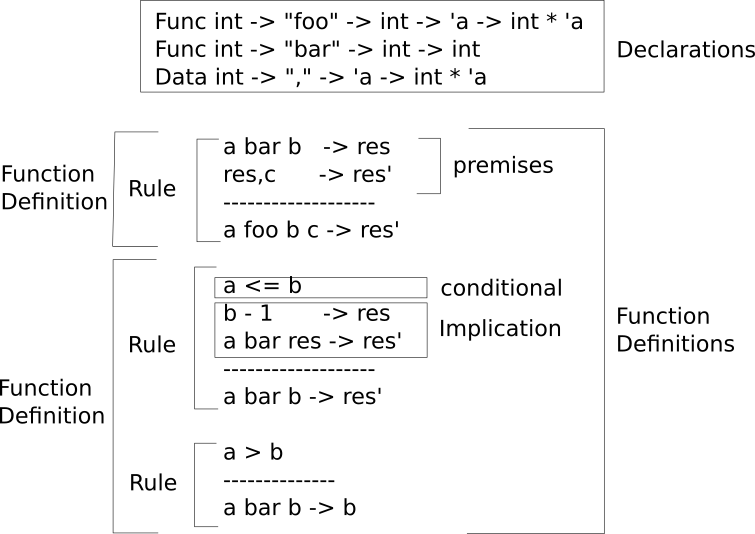
\includegraphics[width=0.7\linewidth]{intro}

\paragraph{}
Now let's go over the different parts:

\paragraph{Declarations}
enable the user to define their own keywords.
The keywords are in parenthesis and the arrows define the order of the declaration.
As shown above it is possible to have functions with variables on the left side of the declaration.
The variable after the final arrow is the return value of the function.

\paragraph{Function definitions}
occur after the declarations.
The rule starts with the input and output below the line of dashes, called the bar.
On the left of the arrow the input is stated and on the right the output.
Above the line are where the function actually does the work.
It tests the premises to see if the rule can be executed.
Within the premises you can have clauses, which are tested, and function calls, which are recursively evaluated and fail if they do not return a result.

We can define multiple rules per function and they will be simultaneously executed.
The program will split and rules that don't match will stop.

\paragraph{Data and Func}
are both used to declare. Func defines a function and Data defines a data type.
The major difference between them is that Data is two-way traversable and Func only one-way.
This means that when we have a variable which has a type created by Data we can extract the start values.
We cannot do this with Func.
Func also has the ability to curry, but both however define terms by using types.\footnote{For more information about terms and types see \cite{pierce2002types}}

\subsubsection{Going higher}
Take a look at the following source code:

\paragraph{}
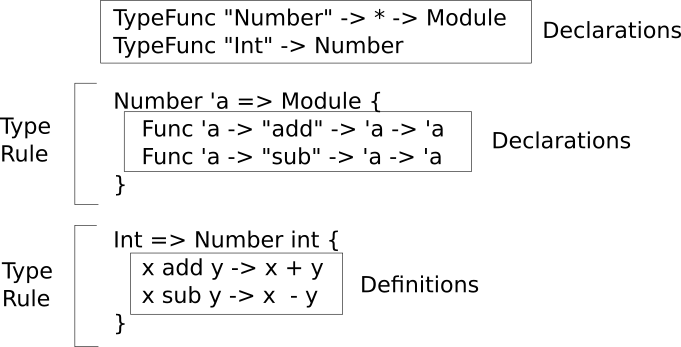
\includegraphics[width=0.7\linewidth]{module}

\paragraph{}
Here we see a similarity with the previous code example.
There are again declarations and rules, this time however we also see a declaration in a rule.
Let's go over the new keywords one by one.

\paragraph{TypeFunc}
is similar to Func in that it declares.
However, as the name suggests, TypeFunc defines a type and not a term.
And it uses kinds to do this.\footnote{For more information about kinds see \cite{pierce2002types}}
These types can than be implemented by Func as we can see in the example.

Another difference is the arrows used.
Instead of using the normal arrow (->) the => arrow is used in TypeFunc declarations.
This is to add clarity as to what is being declared.

\paragraph{Module}
is used to create a collection of declarations.
In this case two Func declarations are used.
We can also use the TypeFunc or Data declarations within a module.

When we take the example module Number, we can see it takes an argument.
As we can see in the Func declarations it is implied that this argument is a type and not a variable.
These variables are called type-variables and are distinguishable by an apostrophe at start of their name.

The declaration of "add" and "sub" within Int assume that the + and - operators are already defined.
We will later see how to use built-in and system operators in section \ref{sec:system}.
Because Int makes use of the module Number by feeding it a type-variable, there is no need for declarations of "add" and "sub."
They exist within the module Number and can thereby be used by any definition of the Number.





%USE THIS SOMEWHERE LATER



%\subsubsection{going without definition}
%In the following source code we something new, namely a lambda:
%insert third picture of oarno

%$\left.\begin{minipage}{5cm}
%\begin{lstlisting}
%(\ x ->
%x + 4 -> res
%res -2 -> res'
%res') -> lam
%\end{lstlisting}
%\end{minipage}\right\rbrace$ test drie
%\begin{lstlisting}
%----------------
%bar -> lam
%\end{lstlisting}


\paragraph{Lambdas}
are defined by:

\begin{lstlisting}
(\ variables ->
do stuff) -> input\_for\_lambda
\end{lstlisting}

(TODO)

\subsection{Standard Library}
Now let's have a look at what is in the standard library and explain some more functionalities of MC.
The standard library consists of the following:
\begin{multicols}{2}
   \begin{enumerate}
      \item StandardLibrary
         \begin{enumerate}
            \item boolean
            \item monad
            \item tryableMonad
            \item number
            \item newnumber
            \item match
            \item prelude
            \item record
         \end{enumerate}
      \item BasicMonads
         \begin{enumerate}
            \item either
            \item id
            \item list
            \item option
            \item result
            \item state
         \end{enumerate}
   \end{enumerate}
\end{multicols}

\subsubsection{System-links}\label{sec:system}
System-links refer to the .NET libraries which are implemented within MC.
When we take a look at boolean we can see how system-links are implemented within MC:

\begin{lstlisting}
TypeFunc "Boolean" => Module
Boolean => Module {
   Func "True" -> Boolean^system
   Func "False" -> Boolean^system
}
\end{lstlisting}

First we specify which system-links we want to implement after which we tell MC it is a system-links.
Using this manner of loading system-types we don't have to write everything from scratch and quickly build upward.

Of course this only tells MC that true and false are of type boolean.
MC still doesn't understand which value they have.
For this we simply implement the Boolean Module, as is done in prelude:

\begin{lstlisting}
import boolean

Boolean => Boolean {
   True -> TrueBoolean^system
   False -> FalseBoolean^system
}
\end{lstlisting}

First we import the Boolean Module from the file boolean.
Then we implement Boolean and tell which term True and False will get.
Because of scoping we con use the same name for Boolean as the Module name for Boolean.

\paragraph{}
When we look at Monad and TryableMonad we see a few new keywords as well as a more complex practical application of MC.

\subsubsection{Monad}

\begin{lstlisting}
import prelude

TypeFunc "Monad" => (* => *) => Module
Monad 'M => Module {
   ArrowFunc 'M 'a -> ">>=" -> ('a -> 'M 'b) -> 'M 'b   #> 10 L
   Func "return" -> 'a -> 'M 'a

   Func "MCons" -> *
   MCons -> 'M

   Func "returnFrom" -> 'a -> 'a
   returnFrom a -> a

   Func "lift" -> ('a -> 'b ) -> 'M 'a -> 'M 'b
   a >>= a'
   --
   lift f a -> return(f a')

   Func "lift2" -> ('a -> 'b -> 'c) -> 'M 'a -> 'M 'b -> 'M 'c
   a >>= a'
   b >>= b'
   --
   lift2 f a b -> return(f a' b')

   TypeFunc "liftM" => (* => *) => * => *
   N >>= a
   f a -> b
   lift^N(return^N b) >>= res
   --
   liftM f N -> return res
}
\end{lstlisting}

\paragraph{}
In Monad the first thing we see is a TypeFunc which tells MC what exactly a monad is.
It takes as an argument "( * => * )" and returns a Module.
As we have explained in \cite{sectionstuff}
a Module is used as a container.
With this in mind a Monad is nothing but a collection of declarations which takes an argument.

When we look at the argument it takes we notice it is a function of some sort which takes a type and returns a type.
Which in kinds are described as *.

The 'M stands for a monad it takes.
This might be confusing if you have any knowledge about monads, since monads are not always a function.
That's because Monad is actually a basis for monad transformers.
As we will see in \cite{sectionstuff}, it comes in very handy when working with monads.

But let's first look at the new keywords we see in Monad.

\paragraph{Import}
does what most programmers would expect, it imports the functions from the file specified after "import."

\paragraph{ArrowFunc}
is an abbreviation of Func.
It creates a function which can take arguments placed on the right of the "operator", from the line below it.

It gives an error if the number of right arguments is not met.

At the end of ArrowFunc we see another type of arrow, \#>, the priority arrow.
It gives the possibility to give it a priority and say if it is left- or right associative.
ArrowFunc is standard right associativity, so there is no need to specify that other than clarity.

\paragraph{Comments}
are a simple but essential feature.
They enable the programmer to explain what is happening when the code is complex.
In MC a single comment line starts with \$\$ and when we want to comment a block we use \$* to start and *\$ to end the block.


\subsubsection{TryableMonad}

\begin{lstlisting}
import prelude
import monad

TypeFunc "TryableMonad" => ( * => * ) => Module
TryableMonad 'M => Monad(MCons^M) {
   inherit 'M

   Func "try" ('a -> MCons^'M 'b) => ('e -> MCons^'M 'b) => MCons^'M 'a => MCons^'M 'b

   Data "e" -> String

   Func "getMonad" -> MCons^'M
   getMonad -> 'M

   Func "Tryable" -> 'a -> 'a
   Tryable -> a -> a
}
\end{lstlisting}

Now let's look at what's new in TryableMonad

\paragraph{Inherit}
has a similar functionality as import, but it imports the functions of a variable.
Note that this is only possible if the variable is based on a module, as only a module can contain function definitions and declarations.


\subsection{Monads implemented}

When we look at a basic implementation of the monads in MC, we will see how using monad transformers is much easier in the end.

We will first take a look at the ID monad transformer and then see how this will make the transformers usable.

\begin{lstlisting}
import prelude
import monad

TypeAlias "Id" => * => *
Id 'a => 'a

TypeFunc "id" => Monad

id 'M a => Monad(Id) {
   inherit 'M

   x >>= k -> k x
   return x -> x
}
\end{lstlisting}

\paragraph{TypeAlias}
creates a data type on kind level.
This way we can use Id as a signature to implement the "id" monad.
Without TypeAlias there would be no way of actually implementing a monad.

\paragraph{}
As we can see, having a basic understanding of MC, the id monad does nothing with the input.
This makes it pass the functionality of the input monad transformer directly as output, thus creating the monad itself.

Without having an id monad there would be no way of using the monad transformers, making them pointless.


\subsection{Put to the test}
Now that we have a better understanding of MC, we can put it to the test using the criteria described in section \ref{sec:criteria}.

\begin{multicols}{2}

   \subsubsection{Read- \& Write ability}\label{sec:readwrite}
   \paragraph{Keywords}
   are few and clear in what they do.
   Furthermore we can define our own keywords by using the different declaration methods.\cite{sectionstuff}
   Which means we can basically build our own language which is strongly typed and tuned to our needs.

   \paragraph{Abbreviations and concise notation}
   is quite clear in MC.
   It has almost no shorthand functionality, which makes it clear what is what.
   The notation is also quite clear and kept to a minimum, which does exactly what it should and nothing more.
   This is a quick way to recognize the code structure and it's meaning.

   \paragraph{Comments}
   are implemented in a proper way as shown in \cite{sectionstuff}.

   \paragraph{Layout or format of programs}
   is mostly a fixed layout, like most modern functional programming languages.
   This is a price for having a strong type system.

   \paragraph{No overuse of notation}
   rarely comes into play.
   At most we will see the bars fairly often and declarations quite often.

   \subsubsection{Simplicity}\label{sec:simplicity}
   \paragraph{Structure}
   is one of the stronger points of MC.
   Declarations and there implementation make it so there is a good structure to be made in the source code.
   We can group the declarations together and the implementations or group the declarations together with their implementations.

   \paragraph{The number of features}
   are basic but very expandable.
   This makes it easy to understand even complex programs, when we see how they are build on top of the basics.

   \paragraph{Multiple ways of specification}
   are achievable through declaring them.
   Though the basics of the language is quite strict, we can build almost anything with them.
   So if we want we can declare multiple ways of doing the same thing.

   \paragraph{Multiple ways of expressing}
   are achievable by overloading the standard operators or declared operators.
   This can make it very obscure what is actually done, but gives us the freedom to create and tune our own operators.

   \subsubsection{Definiteness}
   Definiteness is definitely there, but not completely realised yet.
   At least the parser monad should be implemented in the standard library.
   And to be really sure an example compiler would be handy or some proper documentation.

   All the basics are there to realize the goal of MC, it just needs to be implemented.

   \subsubsection{Orthogonality}
   Orthogonality is probably one of the things MC aims to achieve the hardest with it's type system.
   This has definitely been achieved.
   The strong type system which makes use of three levels: terms, types and kinds.
   Makes sure the language is similar in predictability as languages such as Ada.

   \subsubsection{Expressiveness}
   Expressiveness is quite high because of the high level of abstraction in MC.
   This enables us to express very complex ideas with very little and clear code.

   \subsubsection{Efficiency}
   Efficiency is something we can't really test without a fully functional compiler.
   For we cannot test this.
   For more on this subject see \cite{jarnoshizzle}

   \subsubsection{Libraries}
   Libraries are definitely lacking at this moment in time.
   This only concerns the StandardLibrary, the link with .NET makes the libraries considerably stronger.

   \subsubsection{Hackability}
   Hackability is a big part of MC, we can create the language we want.
   MC itself can be quite powerful by itself, but it really shines when we build a compiler for the language we had in mind.

   This might be quite a big step for a lot of programmers, but it can be very productive if they try it.
   It can save them time in the end.

   \subsubsection{Succinctness}
   Succinctness is something MC falls short.
   We have to declare every function we will ever make, which is anything but succinct.
   But as with Ada and Haskell, we have compromise something for a strong type system.

   \subsubsection{Redesign}
   Redesign is also a critical point in MC.
   Because of the declarations needed, we will have to redo those entirely when rewriting or redesigning.
   On the other hand, we can edit the implementation of a certain declaration any way we want, ass long as the input and output work the same way.

   MC definitely has not been made for evolutionary programming.
   It's more of a think-before-you type language.

   \subsubsection{External Factors}
   External  seem to be promising for MC.
   The main advantage MC has is the interface with the .NET libraries.
   This enables native compatibility on the Microsoft Windows platforms and via Mono it, can also work on the GNU/Linux platforms.

\end{multicols}
